\subsection{Content Filtering}
The implementation of content filtering constitutes of Python scripts which handle all of the data preprocessing, training of the model and predicting of the post categories. As with abuse detection, this makes use of multiple Python libraries including Sci-kit learn \cite{scikit:home}, NLTK \cite{nltk}, Numpy \cite{Numpy} and Pandas \cite{Pandas}, which provide machine learning models and objects for processing datasets. The code is divided between three files, each of which handle a stage of the machine learning process: preprocess.py, train.py and predict.py.

\subsubsection{Data Description}
Although in the future, Fidelis posts will be used to train the model, until there is sufficient data stored by Fidelis, a training set from Twitter is used, as discussed in section \ref{sec:training-data}. This training set contains two attributes: Tweet text and category. The categories in the category column correspond to the default main categories which are used on the discover page, which are: Arts, Business, Education, Games, Health, Home, News, Recreation, Science, Shopping, Society, Sport and Technology. There are 59010 Tweets in the dataset. The graph in figure \ref{fig:category-spread} shows the number of Tweets belonging to each category in the dataset, with arts being the most prevalent with 6680 Tweets and shopping the least with 693 Tweets.

\begin{figure}[H]
\centering
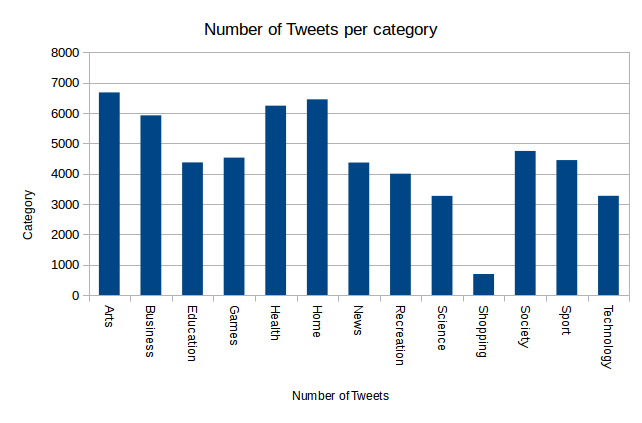
\includegraphics[width=\textwidth]{Images/Implementation/category-spread}
\caption{Spread of Tweets over categories in training set}
\label{fig:category-spread}
\end{figure}

\subsubsection{Data Preprocessing}
The file preprocess.py cleans the textual post so that it can be used in either the training or predicting processes. The implementation of the cleaning is shown in figure \ref{fig:content-clean}. The function carries out a list of commands sequentially, each of which remove aspects of the post which are unwanted. The package \textit{p}, whose \texttt{clean()} function is used is the tweet-preprocessor package \cite{TweetPreprocessor}. This function removes any Twitter entities, except for the hashtags, from the post, including mentions, URLs and emoticons. Since Fidelis is using the same tagging system as Twitter, the same cleaning function can be applied to Fidelis posts. The $WordLemmatizer$ object is from the NLTK library, which processes lemmatizes each of the words in the post to reduce the noise created as a result of different forms of the same word. 

\begin{figure}[H]
\centering
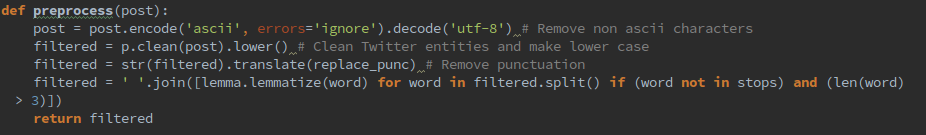
\includegraphics[width=\textwidth]{Images/Implementation/content-clean}
\caption{Function that cleans a post}
\label{fig:content-clean}
\end{figure}

The only part of the design algorithm \ref{alg:content-filter-cleaning} which is not performed by this function is the check that the length of the preprocessed string is less than 20. This is instead performed by both the training and prediction functions. Figure \ref{fig:content-preprocess} shows the preprocessing which occurs in the training file.

\begin{figure}[H]
\centering
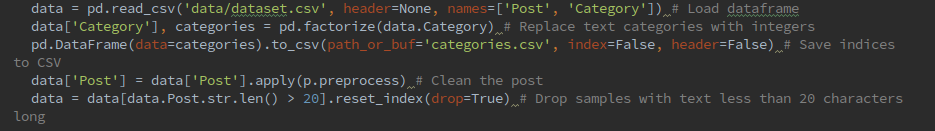
\includegraphics[width=\textwidth]{Images/Implementation/content-preprocess}
\caption{Preprocessing of content before training}
\label{fig:content-preprocess}
\end{figure}

In addition, the extraction of features from the post is performed in the training and prediction files, because they are performed on the dataset as a whole rather than on each individual post. The count vectorization and tf-idf transformations are parsed into the pipeline shown in \ref{fig:imp-content-train}, using the Sci-kit learn objects $CountVectorizer$ and $TfidfTransformer$ (see \ref{sec:feature-engineering}). The $CountVectorizer$ also creates the uni- and bi-grams which are present in the dataset.

\subsubsection{Model Building}
Figure \ref{fig:imp-content-train} shows how the Stochastic Gradient Descent model is trained, including the pipeline which extracts features from the dataset. Whereas the pipeline stage creates the model, the \texttt{fit()} function is what initiates the training of the model on the training data. As with in section \ref{sec:exporting}, the trained models can then be exported so that they can be used to predict incoming tags and posts without having to retrain the model.

\begin{figure}[H]
\centering
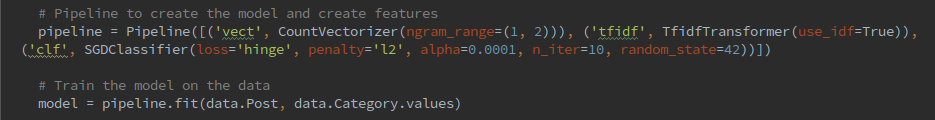
\includegraphics[width=\textwidth]{Images/Implementation/content-train}
\caption{Training the model}
\label{fig:imp-content-train}
\end{figure}

However, as well as building the model using the entire dataset, cross-validation is also implemented, where the model is only trained on 90\% of the data at a time. Figure \ref{fig:content-cv} shows how the cross-validation is performed. This is performed alongside the training of the model in train.py. The function \texttt{cv\_val\_score()} is imported from Sci-kit learn, and handles the splitting of the dataset and the training/testing of each cross-validation model to calculate the score.

\begin{figure}[H]
\centering
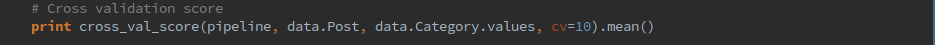
\includegraphics[width=\textwidth]{Images/Implementation/content-cv}
\caption{Cross-validating the model}
\label{fig:content-cv}
\end{figure}

\subsubsection{Predicting Topics}
The categories of the tag are predicted every 15 minutes by the execution of a scheduled program. This Python script, which is in figure \ref{fig:predict-tag} collects all the tags from the tags table where the categorised attribute is set to 0. These uncategorised tags are then passed to the imported classification model, which predicts which category the tag belongs to. Finally, the database is updated and the category-tag pairs are added to the category\_tags table so that they can be used by the discover page. Interactions with the database are handled using a MySQL cursor from the MySQL package. The cursor is open throughout the execution of the script until is closed at the end of the prediction process. All of the tags which are collected from the database are stored in a Pandas dataframe so that it can be passed to the machine learning model. In addition, the category.csv file is imported, which contains the mappings from the integer values representing the categories in the trained model and the actual name of the category.

\begin{figure}[H]
\centering
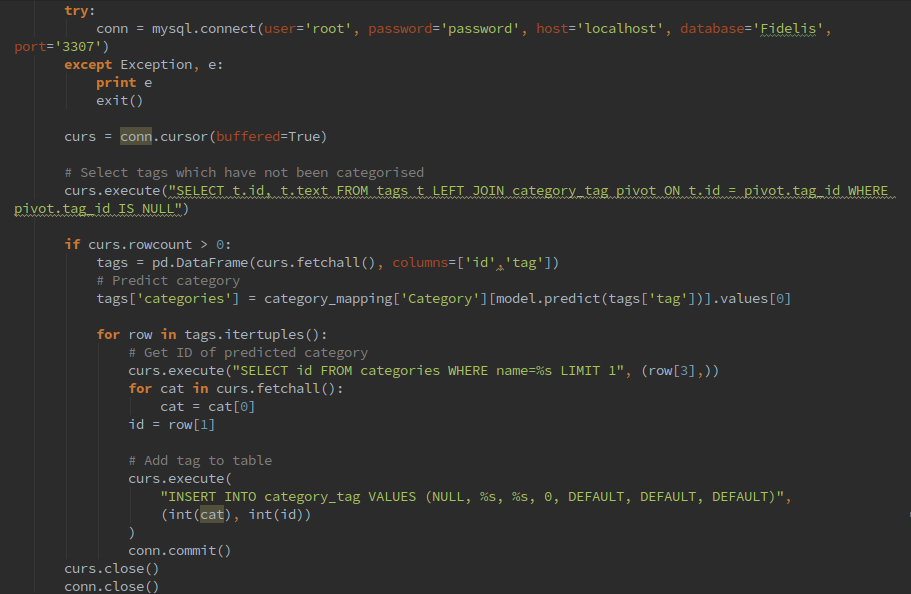
\includegraphics[width=\textwidth]{Images/Implementation/predict-tag}
\caption{Predicting the tag's category}
\label{fig:predict-tag}
\end{figure}

Post categories are predicted using the API, which makes a call to the PostController function \texttt{predict()} after a post has been made. As shown in figure \ref{fig:predict-api}, the function attaches the post to the tag which represents the category. Because the model used to predict the post is a Python script, the PostController uses the $Process$ object to run the script and retrieve the predicted category which is output by the script. After attaching the post to the tag, and thus adding the post-tag pair to the post\_tag table, the API returns the post's category so that JavaScript can be used to update the category on the user's display. 

\begin{figure}[H]
\centering
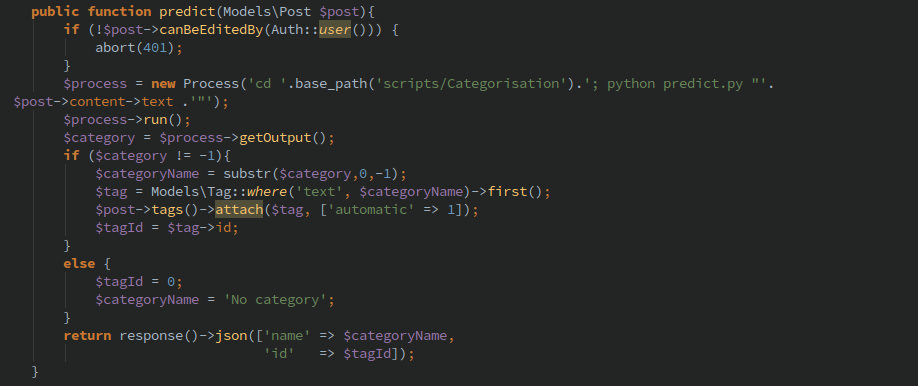
\includegraphics[width=\textwidth]{Images/Implementation/predict-api}
\caption{API controller for predicting a post}
\label{fig:predict-api}
\end{figure}

The code in figure \ref{fig:predict-post} shows Python script which is used to predict the category of the post. As with figure \ref{fig:predict-tag}, the code is stored in the predict.py file, but the two sections are distinguished by whether a post ID argument is passed when executing the script or not. This part of the script does not use MySQL cursors because any processing involved with the database is handled in the PostController. 

\begin{figure}[H]
\centering
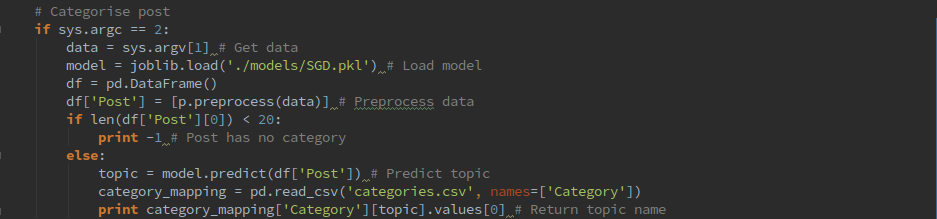
\includegraphics[width=\textwidth]{Images/Implementation/predict-post}
\caption{Predicting a post's category}
\label{fig:predict-post}
\end{figure}

Once the post has been categorised, the user would then be able to change this category in the event that the post has been misclassified. This may be the case when the post does not belong to a category, because the model will always predict that the post belongs to one of the 13 categories even if it is miscellaneous (unless the preprocessed post contains less than 20 characters). The updating of the category is performed by the API once the user has selected a new category using the Bootstrap modal shown in figure \ref{fig:category-modal}. 

\begin{figure}[H]
\centering
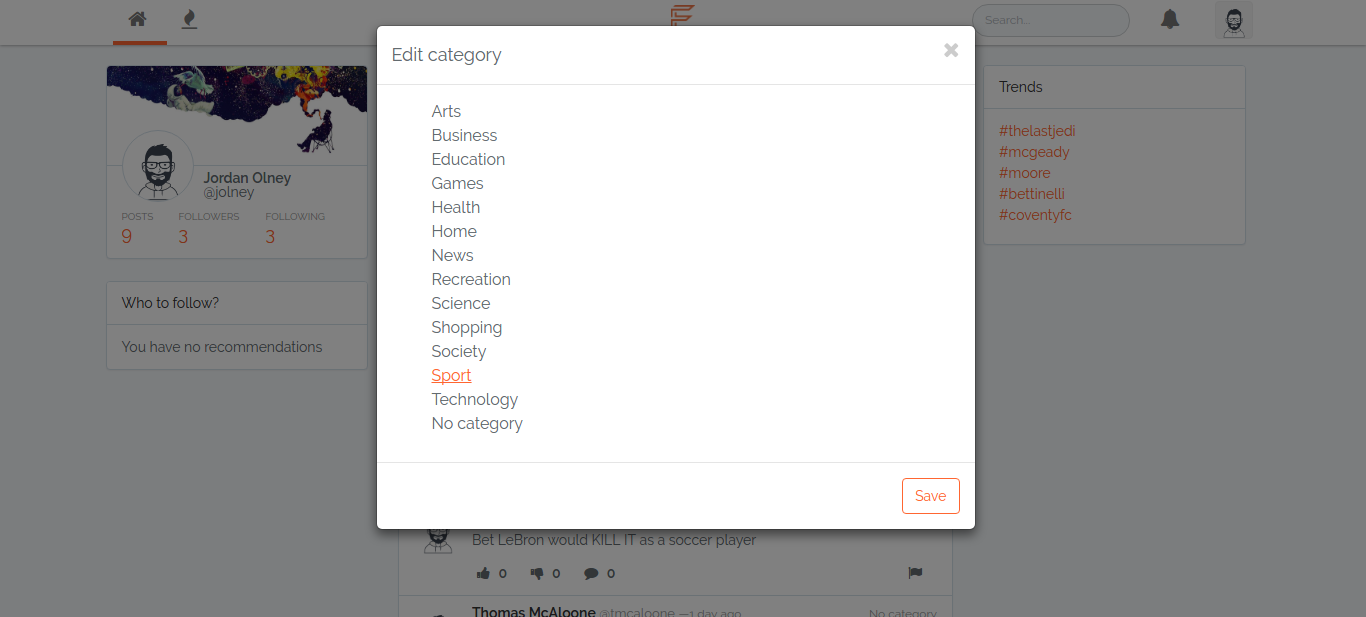
\includegraphics[width=\textwidth]{Images/Implementation/category-modal}
\caption{Modal to edit post category}
\label{fig:category-modal}
\end{figure}

The API request passes the relevant post and (new) category IDs to the \texttt{editCategory()} function in the PostController, which is shown in figure \ref{fig:edit-category}. This function removes the old category from the post\_tags table and replaces it with the new one. The API then returns the new category name to the application front end so that the changes can be reflected in the user interface. 

\begin{figure}[H]
\centering
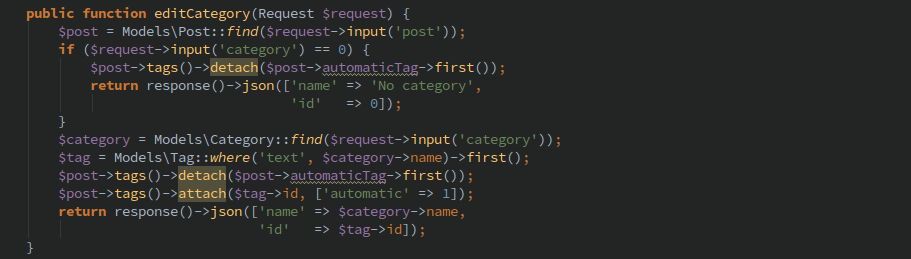
\includegraphics[width=\textwidth]{Images/Implementation/edit-category}
\caption{API controller for changing a post's category}
\label{fig:edit-category}
\end{figure}

